% \pagebreak[4]
% \hspace*{1cm}
% \pagebreak[4]
% \hspace*{1cm}
% \pagebreak[4]

\chapter{Vector hóa văn bản - Doc2Vec}
\ifpdf
    \graphicspath{{Doc2Vec/Chapter1Figs/PNG/}{Doc2Vec/Chapter1Figs/PDF/}{Doc2Vec/Chapter1Figs/}}
\else
    \graphicspath{{Doc2Vec/Chapter1Figs/EPS/}{Doc2Vec/Chapter1Figs/}}
\fi

Từ những gì đã trình bày ở trên, ta hoàn toàn có thể xây dựng được một model word2vec. Tuy nhiên trong bài toán phân loại văn bản, đơn vị của chúng ta là văn bản, không phải từ. Vì vậy cần phải vector hóa văn bản chứ không phải là từ. Chương này sẽ cho chúng ta cách sử dụng mô hình word2vec để xây dựng mô hình Doc2Vec - mô hình ta sẽ sử dụng trực tiếp trong bài toán phân loại văn bản. 
\section{Khái quát về doc2vec} 

Doc2Vec hay còn gọi là Paragraph Vector là phương pháp được trình bày trong Distributed Representations of Sentences and Documents \cite{DBLP:journals/corr/LeM14}. Có thể nói doc2vec là một bản mở rộng của word2vec. Về mặt tư tưởng, word2vec và doc2vec gần như hoàn toàn giống nhau. Nếu như trong word2vec, context đầu vào chỉ là các từ thì ở trong doc2vec context đầu vào có thể chứa các cụm từ, câu, thậm chí là văn bản.

Trong doc2vec, mỗi một paragraph(có thể cụm từ, câu, văn bản) được ánh xạ thành một vector thống nhất đại diện bởi một hàng trong ma trận $D$; còn word(từ) được ánh xạ thành một vector, đại diện bởi một hàng trong ma trận $W$. Paragraph vector và word vector được nối hoặc tính trung bình để dự đoán từ tiếp theo trong một context.  

\begin{figure}
  \begin{center}
    %\leavevmode
    \ifpdf
      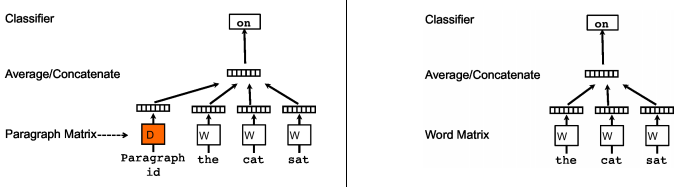
\includegraphics[scale=0.8]{docvsword}
    \else
      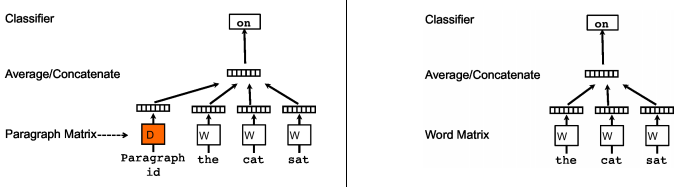
\includegraphics[scale=0.8]{docvsword}
    \fi
    \caption{So sánh doc2vec(trái) và word2vec(phải)}
    \label{docvsword}
  \end{center}
\end{figure}
Hình \ref{docvsword} cho ta cái nhìn trực quan hơn sự khác biệt doc2vec và word2vec. Tuy nhiên, thực tế thì phương pháp xây dựng word2vec và doc2vec không quá khác nhau, nên ta sẽ không đi chi tiết về cách thức xây dựng model này.  